\chapter{Introduzione}
Il \textit{Flusso dei dati} nel front-end di una applicazione web rappresenta tutti gli input e gli eventi che si muovono attraverso i suoi vari livelli logici. Per fare un esempio semplicistico della questione, il banale cliccare su un bottone in un qualsiasi servizio online moderno, fa scaturire un evento che porta con sé dei dati che andranno ad apportare dei cambiamenti nello stato dell'applicazione. Ciascun elemento dell'interfaccia deve successivamente tener conto di questo cambiamento e modificarsi di conseguenza se necessario. Più questo flusso di dati è intenso e disorganizzato, più diventa complicato gestire i cambi di stato e la loro propagazione attraverso tutti i vari componenti.

Un'interfaccia utente quindi mette a disposizione dell'utilizzatore una immensa quantità di interazioni, sia volontarie che involontarie, che cambiano in continuazione lo stato dell'applicazione e che devono essere opportunamente gestite e sincronizzate. La struttura del codice diventa quindi prioritaria al fine di ottenere un prodotto che sia soddisfacente a livello di prestazioni e che riesca a mantenere un adeguato livello di scalabilità.

L'obbietto principale di questa tesi consiste nel fornire una presentazione delle varie architetture e dei vari approcci utilizzati attualmente per risolvere il problema della gestione del flusso di dati in applicazioni web con una codebase solitamente grande e complessa, comparando i loro relativi vantaggi e svantaggi. Verrà effettuata un'analisi approfondita del paradigma \textit{MVC} (Model - View - Controller) lato front-end, spiegando le grosse differenze che si vengono a creare rispetto al suo utilizzo lato back-end e alla sua scarsa scalabilità derivata dall'uso di un flusso di dati bidirezionale tra Model e View. Verranno poi discusse le architetture di \textit{Flux} e di \textit{Redux} che implementano un flusso di dati unidirezionale per ovviare ai problemi del paradigma MVC.
L'analisi coprirà le differenze di implementazione delle due librerie, di come Flux si basi su una struttura complessa ma estremamente funzionale oltre che versatile, e di come Redux la semplifichi attraverso pattern della programmazione funzionale per ottenere lo stesso livello di scalabilità con una semplicità decisamente maggiore.

\section{Background}
La gestione del flusso dei dati all'interno di una applicazione web è un argomento molto discusso dopo l'avvento di tecnologie front-end sempre più complesse e potenti come \textit{React} o \textit{Angular} ma sopratutto con la crescita smisurata della complessità dei servizi online. La causa di ciò è la necessità di avere un codice che sia il più possibile scalabile ed il più facilmente testabile a prescindere dal numero di features che verranno successivamente aggiunte. 

\begin{figure}[h]
\centering 
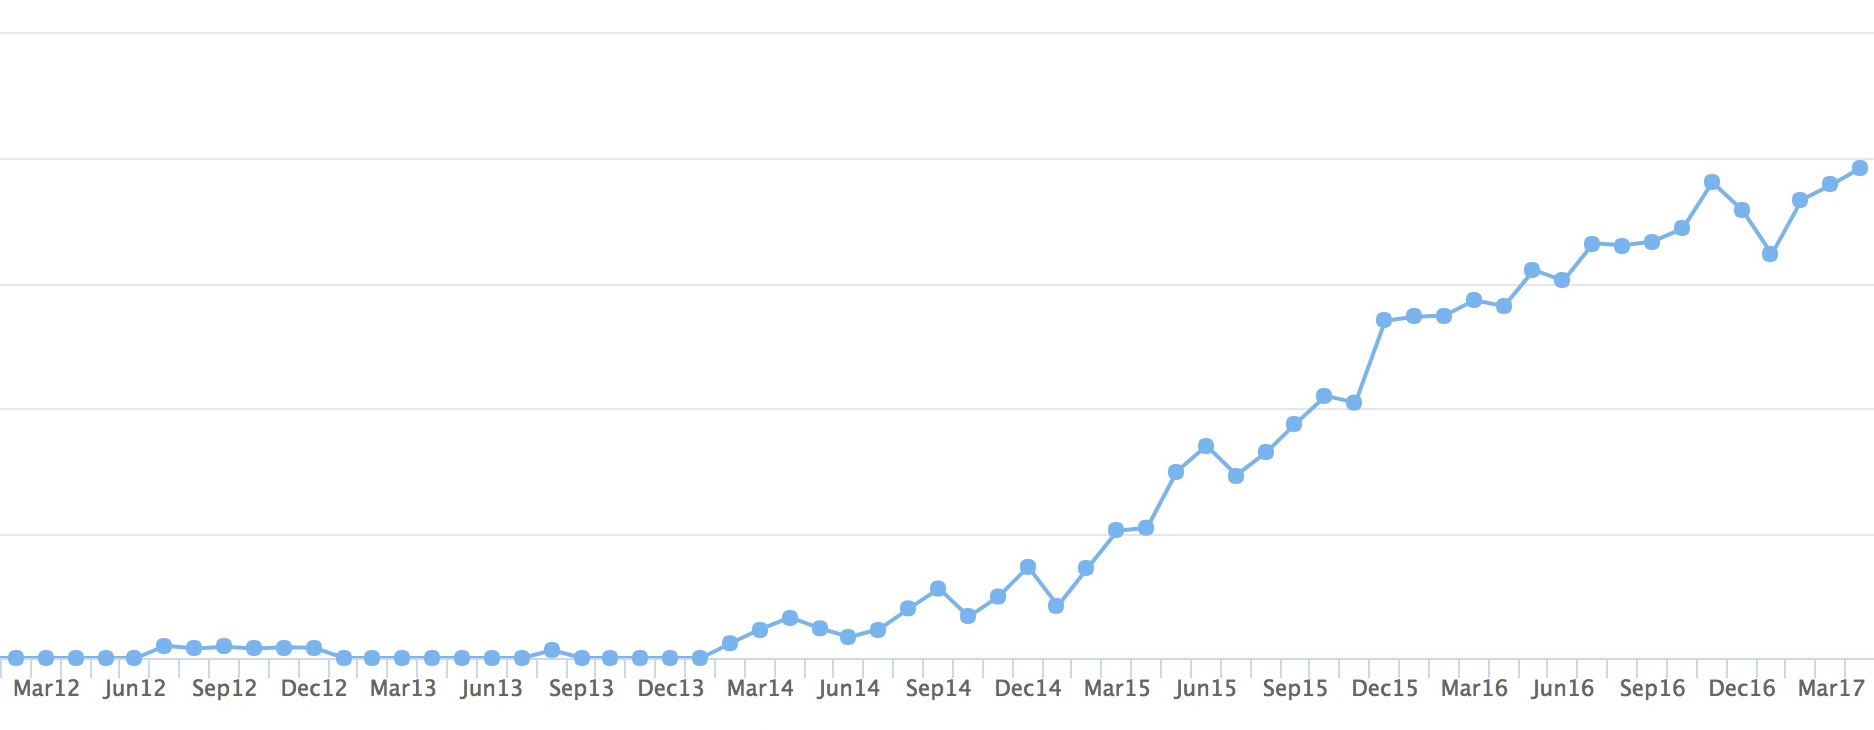
\includegraphics[width=12.7cm]{./images/reactPopularity}
\caption{Grafico della popolarità di React (generato da \href{https://www.hntrends.com/}{hntrends.com}).}
\end{figure}

\noindent
Codebase vaste come potrebbero essere quelle di Facebook, Twitter o YouTube necessitano di una architettura di fondo che sia altamente chiara e comprensibile per evitare confusione tra i vari servizi.
Come vedremo successivamente, architetture datate come l'MVC pur essendo molto efficienti lato back-end non rendono allo stesso modo lato front-end, dove c'è una quantità maggiore di azioni che l'utente può intraprendere e che possono avere ripercussioni differenti su più componenti diversi all'interno di una View.
In questo documento verranno discusse le alternative attualmente più gettonate come quella a flusso unidirezionale, implementata in prima battuta da Flux e successivamente ottimizzata da Redux.

\section{Lo stato dell'arte}
Possiamo paragonare la creazione della prima applicazione web con la messa online del primo sito da parte di Tim Berners-Lee nel 1991 dal Cern di Ginevra \cite{HuffingtonpostFirstWebsite}. Stiamo tuttavia parlando di una applicazione statica costruita solamente in HTML dove gli unici input dell'utente erano limitati al navigare i documenti. Più avanti con l'evoluzione di HTML si iniziarono a vedere i primi elementi interattivi come bottoni e campi di testo. Tuttavia la svolta vera e propria avvenne il 5 maggio del 1995 con l'avvento di Javascript \cite{W3cJavascriptHistory}, il linguaggio di scripting che portò un primo accenno di dinamicità all'interno delle pagine web e che anche adesso è alla base di tutte le tecnologie front-end più nuove e potenti. Da qui in poi l'evoluzione andò avanti in maniera esponenziale partendo da un utilizzo banale del linguaggio fino a giungere alla situazione attuale con framework ed architetture complesse.

\subsection{Single-page application}
Andando avanti con gli anni si sono tentati diversi approcci per la creazione di applicazioni web. Un problema fondamentale è stato quello di dove posizionare la logica del servizio che fino a quel momento è stata sempre considerata come una parte del server specialmente per la mancanza di tecnologie adeguate lato client.

\begin{figure}[h]
\centering
\includegraphics[width=10cm]{./images/noSPA}
\caption{Esempio di una applicazione con la logica nel server.}
\end{figure}

Con la maturazione degli strumenti client-side si è aperta una porta ad un nuovo tipo di applicazioni: le \textit{Single-page application} (SPA). Una Single-page application è una applicazione web contenuta in una sola pagina e che sviluppa tutta la sua logica nel client.

Non è da poco che questo tipo di applicazioni hanno preso piede, tuttavia intorno agli anni 2000 non era Javascript la prima scelta come linguaggio di programmazione ma Flash e Java Applets. Solo più avanti è riuscito a diventare competitivo abbastanza da deprecare entrambi i suoi predecessori per diversi motivi \cite{mikowski2013single}:

\begin{itemize}
    \item \textbf{Velocità di esecuzione} Javascript non ha bisogno di alcun ambiente esterno per essere eseguito consentendo di eliminare un livello di complessità all'applicazione.
    \item \textbf{Nessuna dipendenza esterna} Gli utenti non hanno bisogno di scaricare nessuna dipendenza esterna e quindi nessun plugin per eseguire il servizio.
    \item \textbf{Controllo sulla pagina web} Javascript ha pieno controllo sulla pagina web dove viene eseguito in quanto è tutt'uno con essa. Al contrario, Flash e Java, vengono inseriti in maniera “embedded" nella pagina e non hanno la possibilità di interagire con essa in maniera diretta causando un'esperienza meno fluida ed interattiva per l'utente.
\end{itemize}

\begin{figure}[h]
\centering
\includegraphics[width=10cm]{./images/yesSPA} 
\caption{Esempio di una applicazione SPA.}
\end{figure}

\noindent
La problematica della gestione del flusso dei dati è diventata estremamente rilevante con la comparsa delle SPA in Javascript. Nel loro stadio iniziale queste non erano costruite sopra una struttura ben definita e la gestione del flusso dei dati avveniva in maniera disordinata gestendo ogni azione dell'utente in maniera diretta.
Andando avanti con il tempo e con l'aumentare della complessità di queste applicazioni, si è sentito il bisogno di creare un'architettura ben definita che aiutasse a gestire in maniera più consistente lo stato del servizio e tutti i suoi eventuali cambiamenti.

\subsection{I primi framework basati su MVC}
La necessità di avere struttura più solida lato front-end, specialmente per applicazioni più esigenti, ha portato alla nascita dei primi framework basati sull'architettura MVC.

\blockquote{Single page apps are distinguished by their ability to redraw any part of the UI without requiring a server roundtrip to retrieve HTML. This is achieved by separating the data from the presentation of data by having a model layer that handles data and a view layer that reads from the models. \cite{MixuSinglePageWebApp}}

\noindent Nel modello MVC per front-end (e come anche in quello back-end), che riprenderemo in dettaglio più avanti nel documento, abbiamo una netta distinzione tra i dati dell'applicazione (Model), la presentazione di quest'ultimi (View) e la logica che funge da tramite (Controller), incaricata di gestire gli eventi innescati dall'utente. Questo ci permette di avere un controllo maggiore sullo stato globale e di ogni singolo componente dell'interfaccia oltre ad un codice più robusto e facile da modificare nel tempo \cite{ParrOnTheMVC}.

Javascript ha a disposizione un numero considerevolmente alto di framework MVC, e la maggior parte di questi tendono a sviluppare questa architettura in maniera leggermente differente, con i propri vantaggi e svantaggi a seconda dei cambiamenti che apportano e del tipo di applicazione che si deve costruire.
Una di queste è MVP (Model - View - Presenter) utilizzata da \textit{Backbone.js}\footnote{http://backbonejs.org}. In questa il Presenter, che sostituisce il Controller, ha una responsabilità maggiore di quest'ultimo e oltre che gestire gli eventi dell'utente si occupa di fornire i dati necessari alla generazione della View. Un'altra architettura derivata da MVC è MVVM (Model - View - ViewModel), utilizzata da framework come \textit{Knockout}\footnote{http://knockoutjs.com}, in cui il ViewModel si occupa di mantenere i dati del Model (che sono grezzi) nella forma richiesta dalla View, ed espone a quest'ultima metodi e funzioni per la gestione dello stato dell'applicazione \cite{ChauhanFrontendArchitectures}.

Ancora una volta tuttavia ci troviamo di fronte ad un muro, dove le architetture venutesi a creare sono tante ma tutte derivate da MVC traendone i difetti. Il problema più grande di questo paradigma è la comunicazione bidirezionale: una View, tramite il Controller, modifica diversi Model i quali a loro volta aggiornano le relative View. Tenendo presente che stiamo parlando di applicazioni complesse e quindi con un grande numero di componenti, questo genera un effetto cascata di modifiche tra i vari Model e View causando una codebase molto difficile da gestire ed analizzare. 

Per la prima volta a questo punto si inizia a discutere di flusso di dati in maniera attiva e diretta riconoscendolo come difetto principale del modello MVC e trovando in React la libreria perfetta per risolverlo \cite{SalihefendicFluxVsMVC}.

\subsection{Framework ed architetture a flusso unidirezionale}
Un ulteriore passo avanti nella storia delle applicazioni web è stata React\footnote{https://facebook.github.io/react}, libreria per la creazione di interfacce utente sviluppata da Facebook che si basa su diverse tecnologie all'avanguardia e che permette grazie alla sua versatilità di strutturare architetture più complesse ed efficienti.
React è una libreria e non un framework, ciò significa che il suo lavoro è solamente quello di creare interfacce utente \cite{BunaReactIsTheNewFrontend}. Non è quindi una soluzione finale ma un componente fondamentale che unito ad altri ci permette di scrivere applicazioni web in maniera molto più dinamica.

Per sfruttare al massimo una libreria come React, Facebook mette anche a disposizione una struttura che sembra risolvere il problema relativo alla comunicazione bidirezionale riscontrato nel paradigma MVC. \textit{Flux}\footnote{https://facebook.github.io/flux} è un'architettura complessa per la costruzione di interfacce utente che si basa su un flusso di dati unidirezionale facilmente gestibile ed altamente scalabile. In Flux una View non modifica mai in maniera diretta lo stato di una applicazione, bensì propaga azioni che vengono gestite da un \textit{Dispatcher} e che hanno delle ripercussioni sul Model di questo paradigma che si chiama \textit{Store}. Infine, quest'ultimo si occupa di propagare a sua volta un evento a tutti i componenti delle View che permette loro di aggiornarsi di conseguenza. Questo tipo di approccio di permette di avere un flusso di dati facilmente analizzabile in quanto sappiamo esattamente dove arrivano in input e dove escono in output i dati di ogni singolo strato dell'architettura ma sopratutto ci permette di gestire in maniera chiara e pulita la sincronizzazione tra stato ed ogni singolo componente dell'interfaccia utente.

\subsection{Un approccio funzionale al flusso unidirezionale: Redux}
Flux riesce a risolvere a pieno tutti i problemi fino ad ora descritti causati dalla comunicazione bidirezionale delle architetture MVC e derivate. Tuttavia la complessità di tale paradigma si fa sentire già da subito sia per il gran numero di passaggi che un'azione deve effettuare prima di venire effettivamente eseguita, sia per la difficoltà nell'implementazione anche in applicazioni di medio-piccole dimensioni.

Un'alternativa che si basa sempre su Flux è \textit{Redux}\footnote{http://redux.js.org}, una libreria scritta da Dan Abramov e Andrew Clark che si identifica come semplice “Gestore dello stato" di una applicazione. Redux riesce a semplificare l'architettura di Flux utilizzando dei pattern della programmazione funzionale come la composizione e l'immutabilità per ottenere una struttura a flusso unidirezionale eliminando il Dispatcher e altre complessità \cite{AbramovOnReduxVsFlux}.
Vedremo nei prossimi capitoli come sia semplice ed elegante gestire il flusso dei dati e lo stato di un'applicazione che utilizza Redux e React, e come questi risolvono in dettaglio le principali problematiche delle architetture descritte precedentemente.